%% Hanford investigations

%% TCS schematic for LIGO Hanford for O3
%% TCS pre-loading
 %% Current methodology for tuning TCS
  %% Detail Hanford's methods
 %% Increasing RH tuning speed


%As shown in Chapter 1,  increasing input power leads to a direct increase to the sensitivity of a DRFPMI to make gravitational wave detections. But one implication of this is the necessity for thermal compensation. As the interferometer increases input power, you directly couple more light into the Fabry-P\'{e}rot cavity arms; and even with optics ultra-low absorption ($\approx 400 \; \mathrm{ppb} \pm 150 \; \mathrm{ppb}$ \textcolor{red}{alog ? or point absorber paper}) still induce thermo-optic effects with the projected circulating arm power of 200 kW. A symptom of this is mode mismatch throughout the interferometer, a problem that contributes to loss of usable optical power throughought the DRFPMI which can reduce sensitivity two-fold: loss of power to your readout, and reduced efficacy of the current solution to reduce the quantum noise limit (squeezing).


During O3a circulating arm power reached beyond 180 kW and the potential optical loss from thermo-optic effects at arm powers of this level can cause a reduction in sensitivity (by how much exactly?)). This motivated the thermal compensation system comissioning detailed in this chapter at the LIGO Hanford observatory which includes: a citation and execution of the initial O3 TCS pre-load, the development and implementation of real-time digital filtering for improved ring heater actuation by a factor of $\approx 6$; introducing a dynamic thermal compensator for mode matching actuation and parametric instability, while also applying to the effects of high absorption points aka point absorbers and attempts at mitigating them. 

\section{Pre-loading for O3a}
An inital counter to the thermo-optic test mass response from the self heating that occurs at high circulating arm powers is an initial pre-load of the ring heaters and CO2 lasers. The objective is to maintain the 50 km test mass substrate lens can be roughly preserved while increasing the interferometer input power to the arms. And although estimates of wavefront distortion due to thermal lensing from self heating and ring heater actuation are available and can be computed \cite{Ramette:16, hello_vinet}, they can also be directly measured using Hartmann wavefront sensors sensitive to auxilary beams imaged onto the test mass mirror surfaces. The measured distortion is then mapped in real time to Zernike polynomials with coefficients used to compute the differential thermal lens in diopters.

%\begin{equation}

%\end{equation}

%The presence of high absorption points on the test masses (aka point absorbers) required adjustments to the TCS pre-load and various ring heater and CO2 settings were sampled. Part of this sampling lead to the development of a input ring heater filter allowing actuation to reach ? percent of the desired optical power within 2 hours compared to the 12 hour response pre-filter. Higher spatial frequency actuation in the form of a CO2 mask was also tried.


\begin{figure*}[!h]
  \centering
  \begin{subfigure}{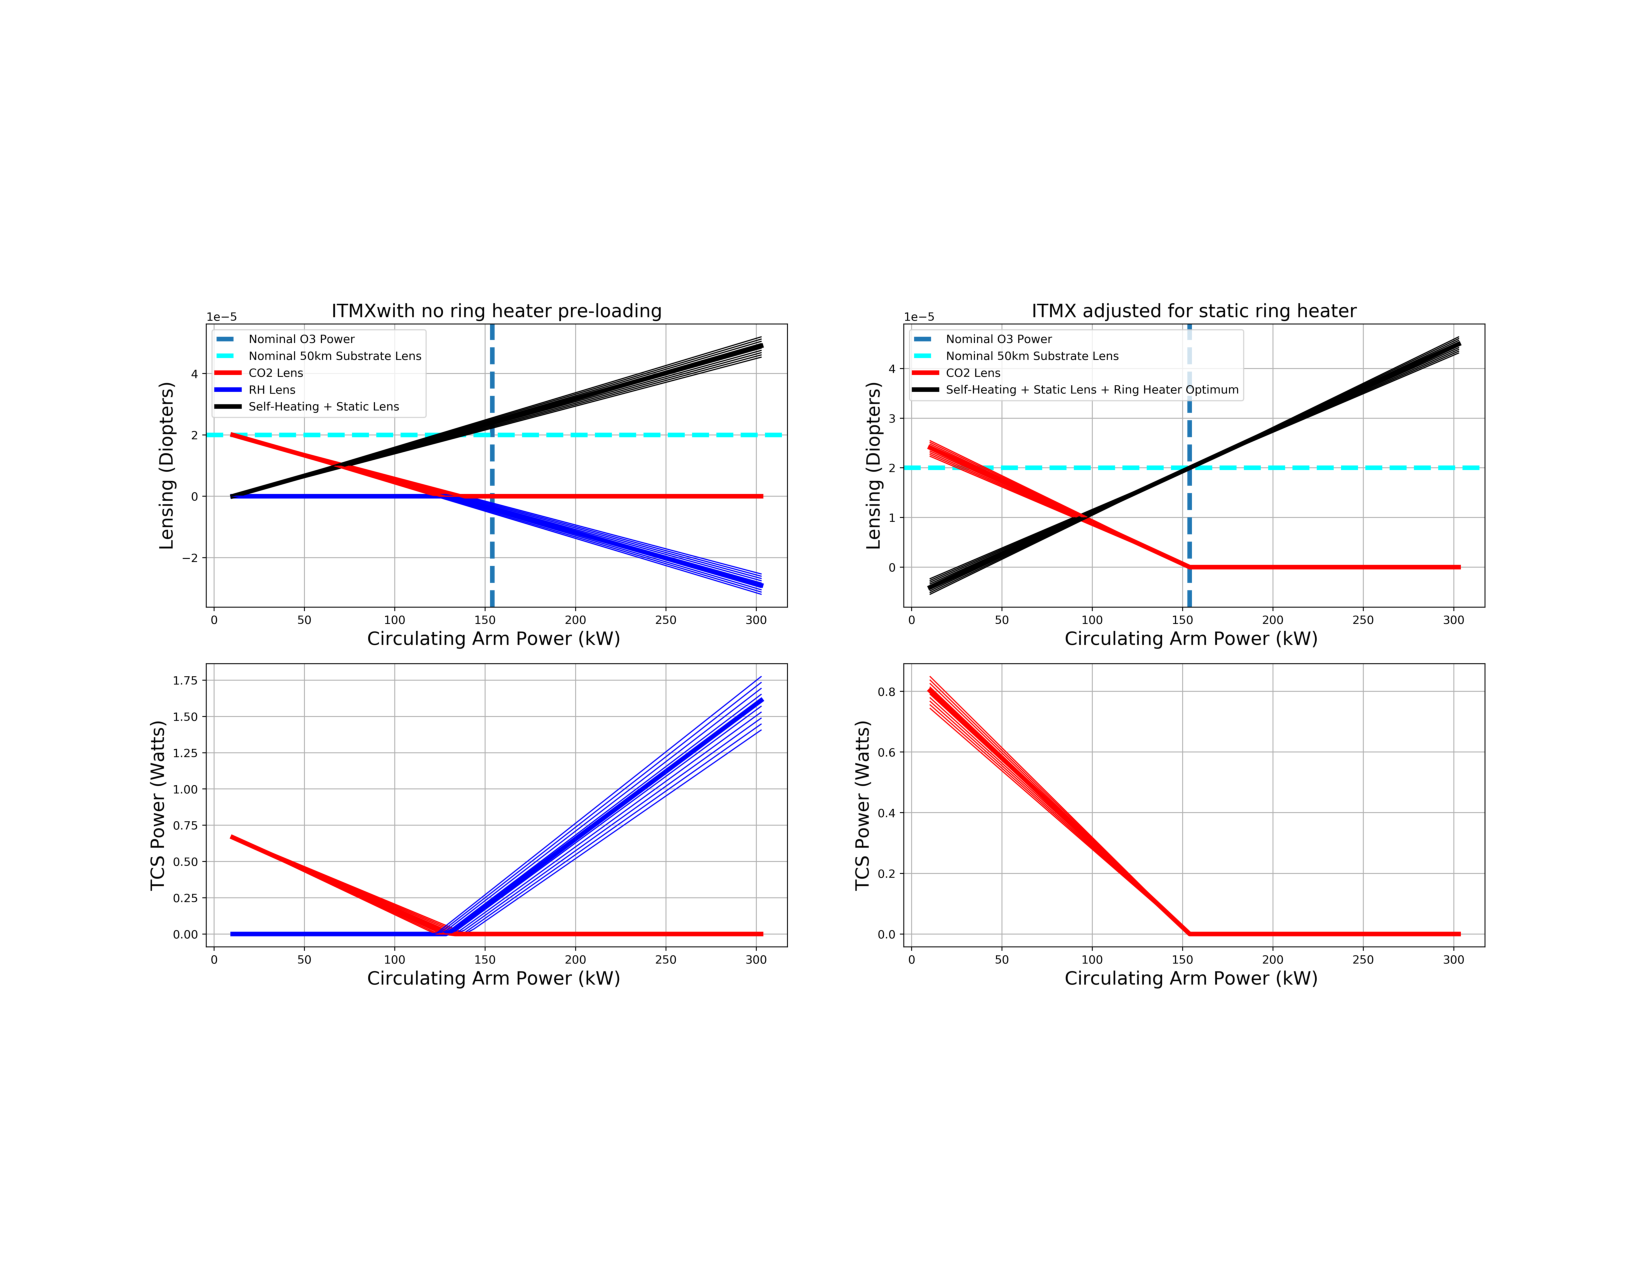
\includegraphics[width=\textwidth]{TCS/ITMX_TCS_Settings_tvo.pdf}}
  \end{subfigure}
  \begin{subfigure}{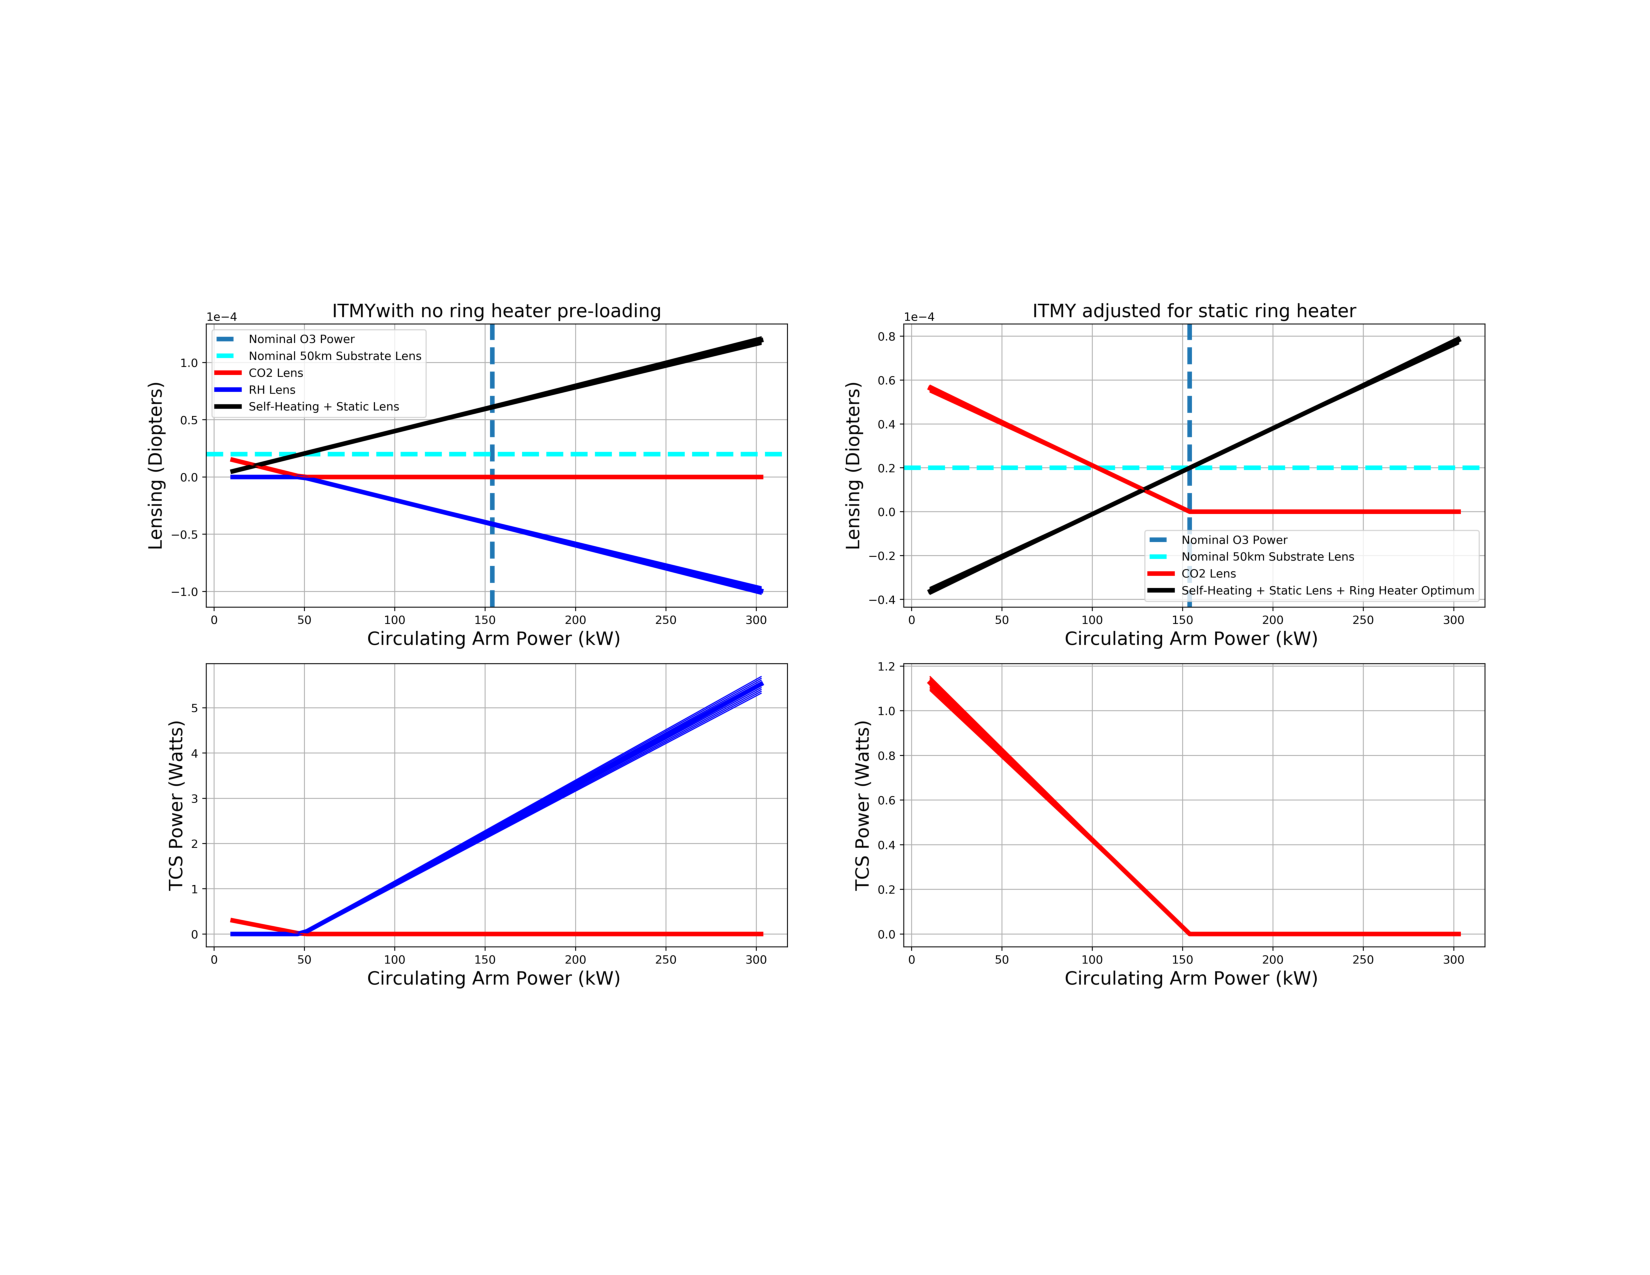
\includegraphics[width=\textwidth]{TCS/ITMY_TCS_Settings_tvo.pdf}}
  \end{subfigure}
  %\begin{subfigure}{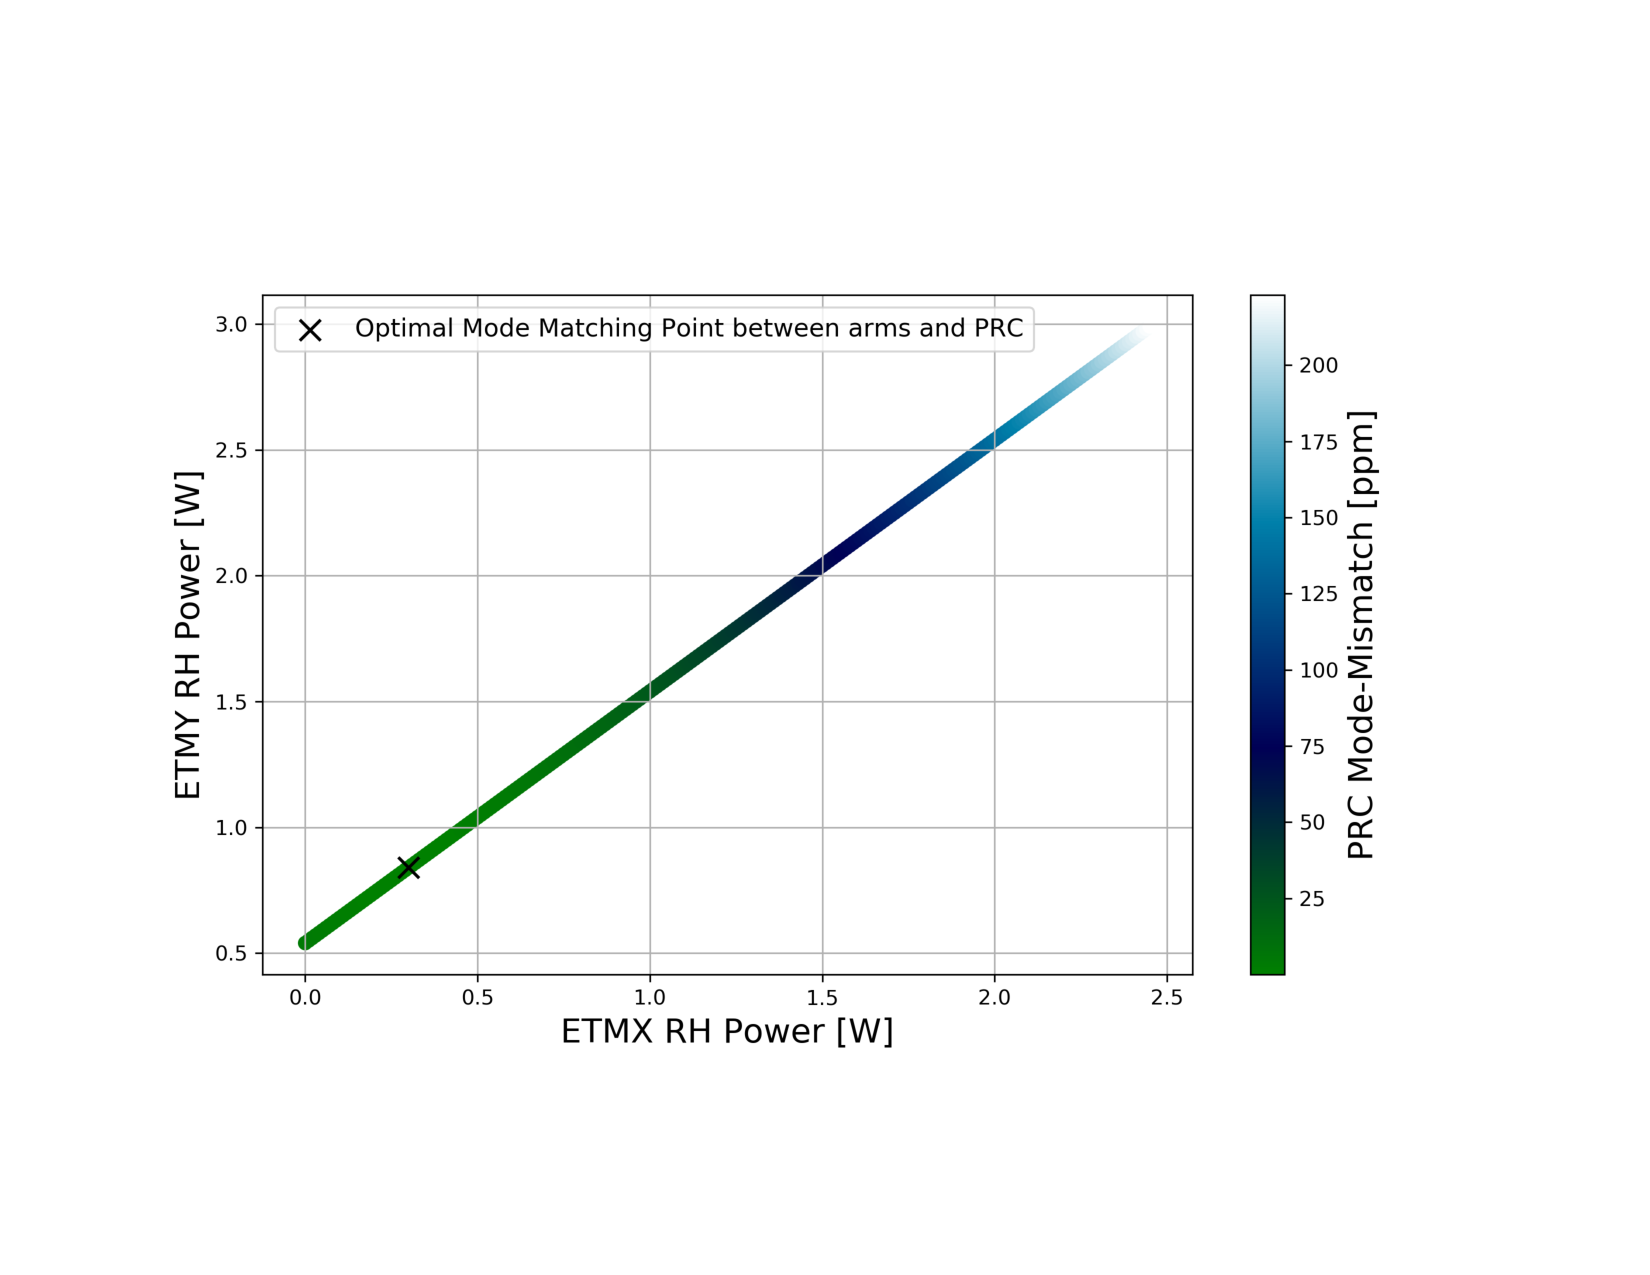
\includegraphics[width=.75\textwidth]{TCS/ETM_TCS_Settings_tvo.pdf}}
  %\end{subfigure}
  \hfill
  \caption{The initial pre-load estimates for the ITMs at the LIGO Hanford Observatory for O3a as provided in \cite{tvo}} 
  \label{fig:O3_preload_tvo}
\end{figure*}

\section{Optimizing RH thermo-optic response}
An analytical model of transient ring heater actuation from a radially symmetric thermal aberration ($\Psi(t,r)$) is realized \cite{Ramette:16}:
\begin{equation}
	\Psi(t,r)=2\frac{dn}{dT} \sum^{\infty}_{m,p = 1} A_{m,p} \; c^{u}_{p} \mathrm{sin}(u_m h /2a) (a/u_m)[1-e^{-\alpha t}] J_0(\zeta_p r/a)
\end{equation}

\begin{figure}[H]
 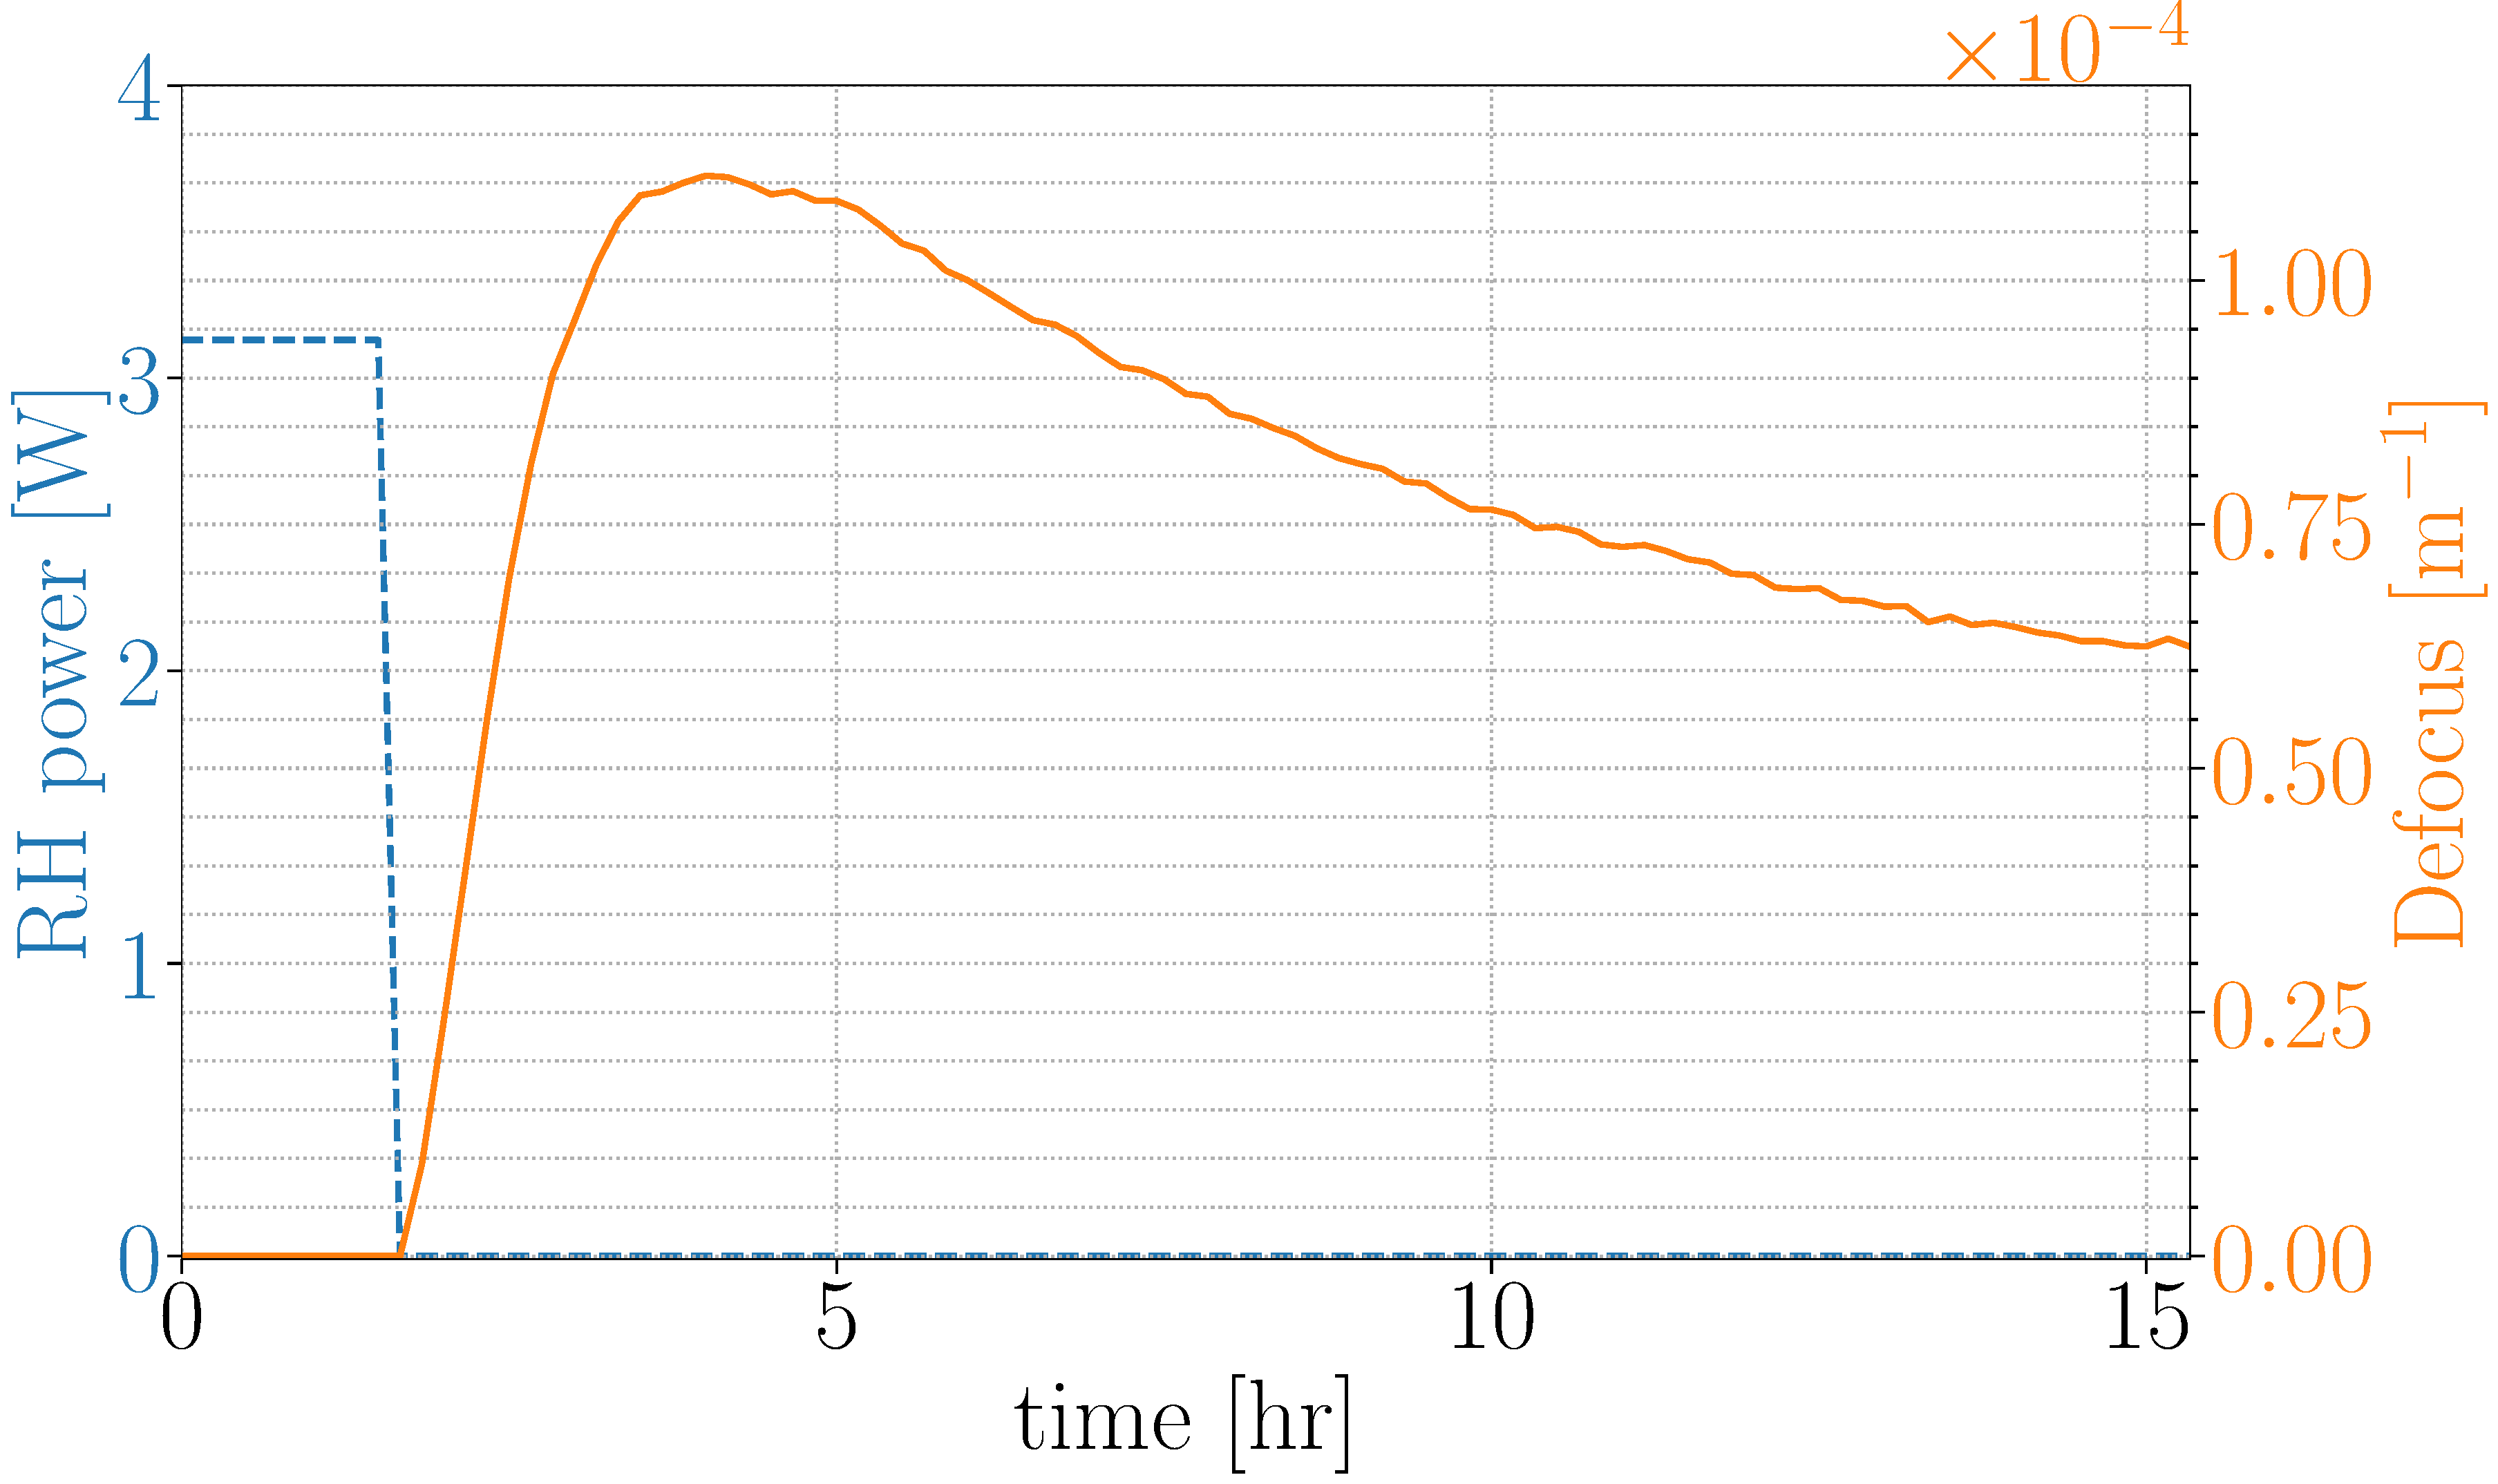
\includegraphics[width=\textwidth]{TCS/IRHF/Meas_response}
 \caption{ITMY thermo-optic response to a 3.13 Watt power reduction to the top and bottom ring heater elements. It's after $\approx$ 12 hours after the change was made do you start to see a small enough $\frac{\mathrm{d} \alpha_\mathrm{sp}}{\mathrm{dt}}$ when you can assume a steady thermal lens.}
 \label{fig:meas}
\end{figure}

The measured transient response can exhibit a prolonged differential defocus on the time scale of $\approx$ 12 to 15 hours; which can make ring heater adjustments another layer of complexity to the comissioning process when leaving the the detector with unideal mode matching conditions for an extended period. Reduced actuation times are possible with the construction and implementation of a real time digital filtering applied to the ring heater input power step.

\begin{figure}[H]
\centering
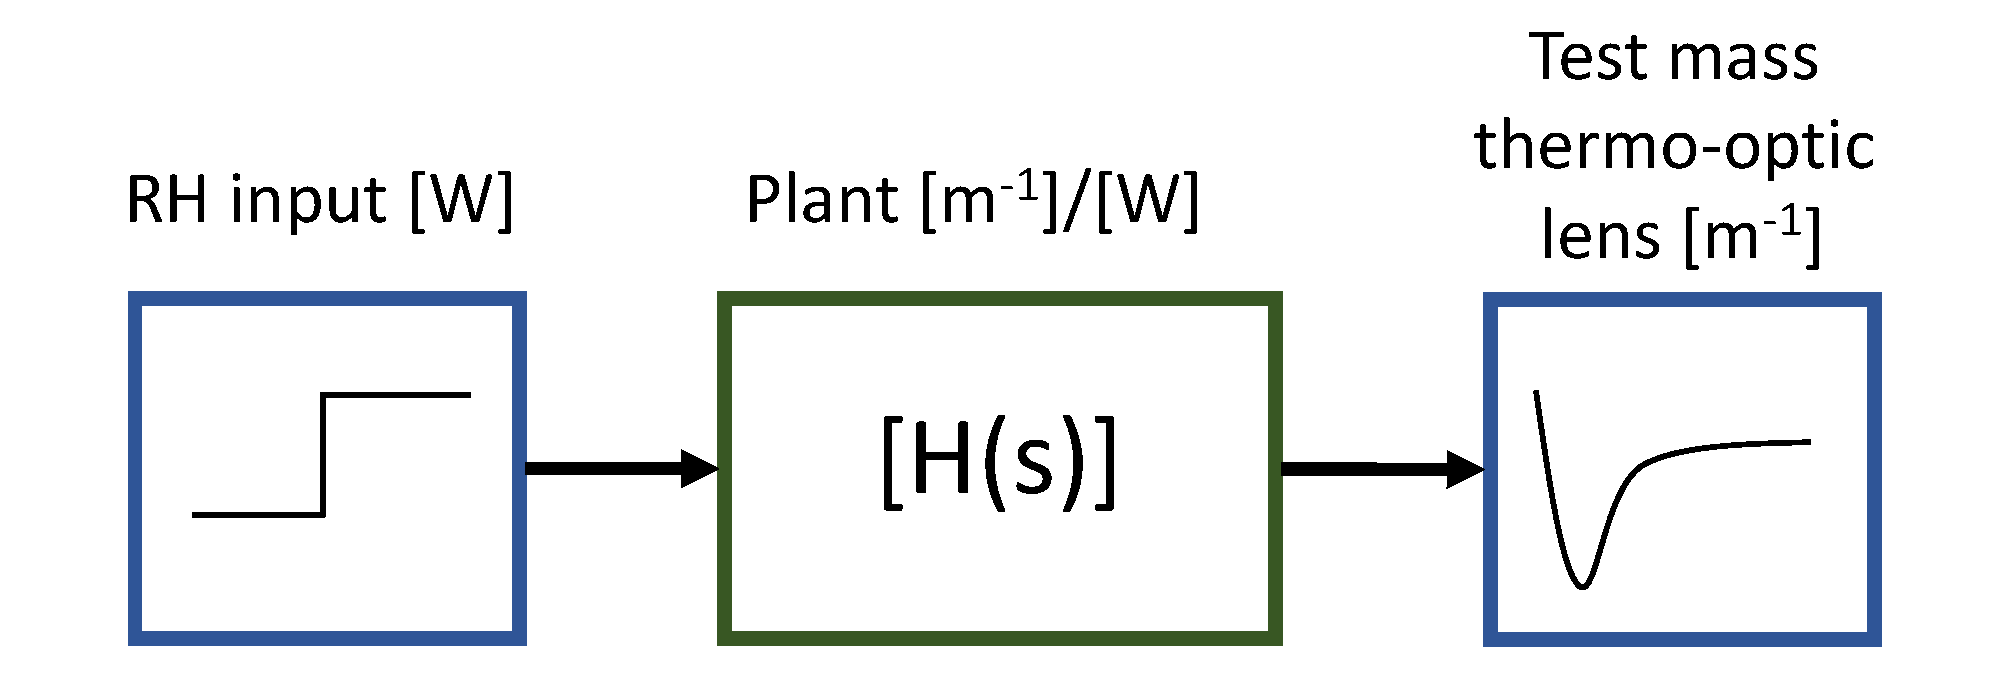
\includegraphics[page=1,width=.75\textwidth]{TCS/IRHF/RH_input_filter_figures.pdf}
\caption{A pictograph showing how the plant transforms the signal. The example of this can be seen in Fig [\ref{fig:meas}]}
\label{fig:justplant}
\end{figure}

The construction of the filter is realized with the following prescription:
%\begin{enumerate}[label=\arabic*),leftmargin=75pt,nosep]
%	\item Fit step response to a zpk filter $H(s)$ 
%	\item Invert fitted filter ($H(s) \rightarrow H^{-1}(s)$) 
%	\item Apply correction filter $G(s)$ for stability and speed tuning ($H^{-1}(s)*G(s)$)
%\end{enumerate}


\begin{figure}[H]
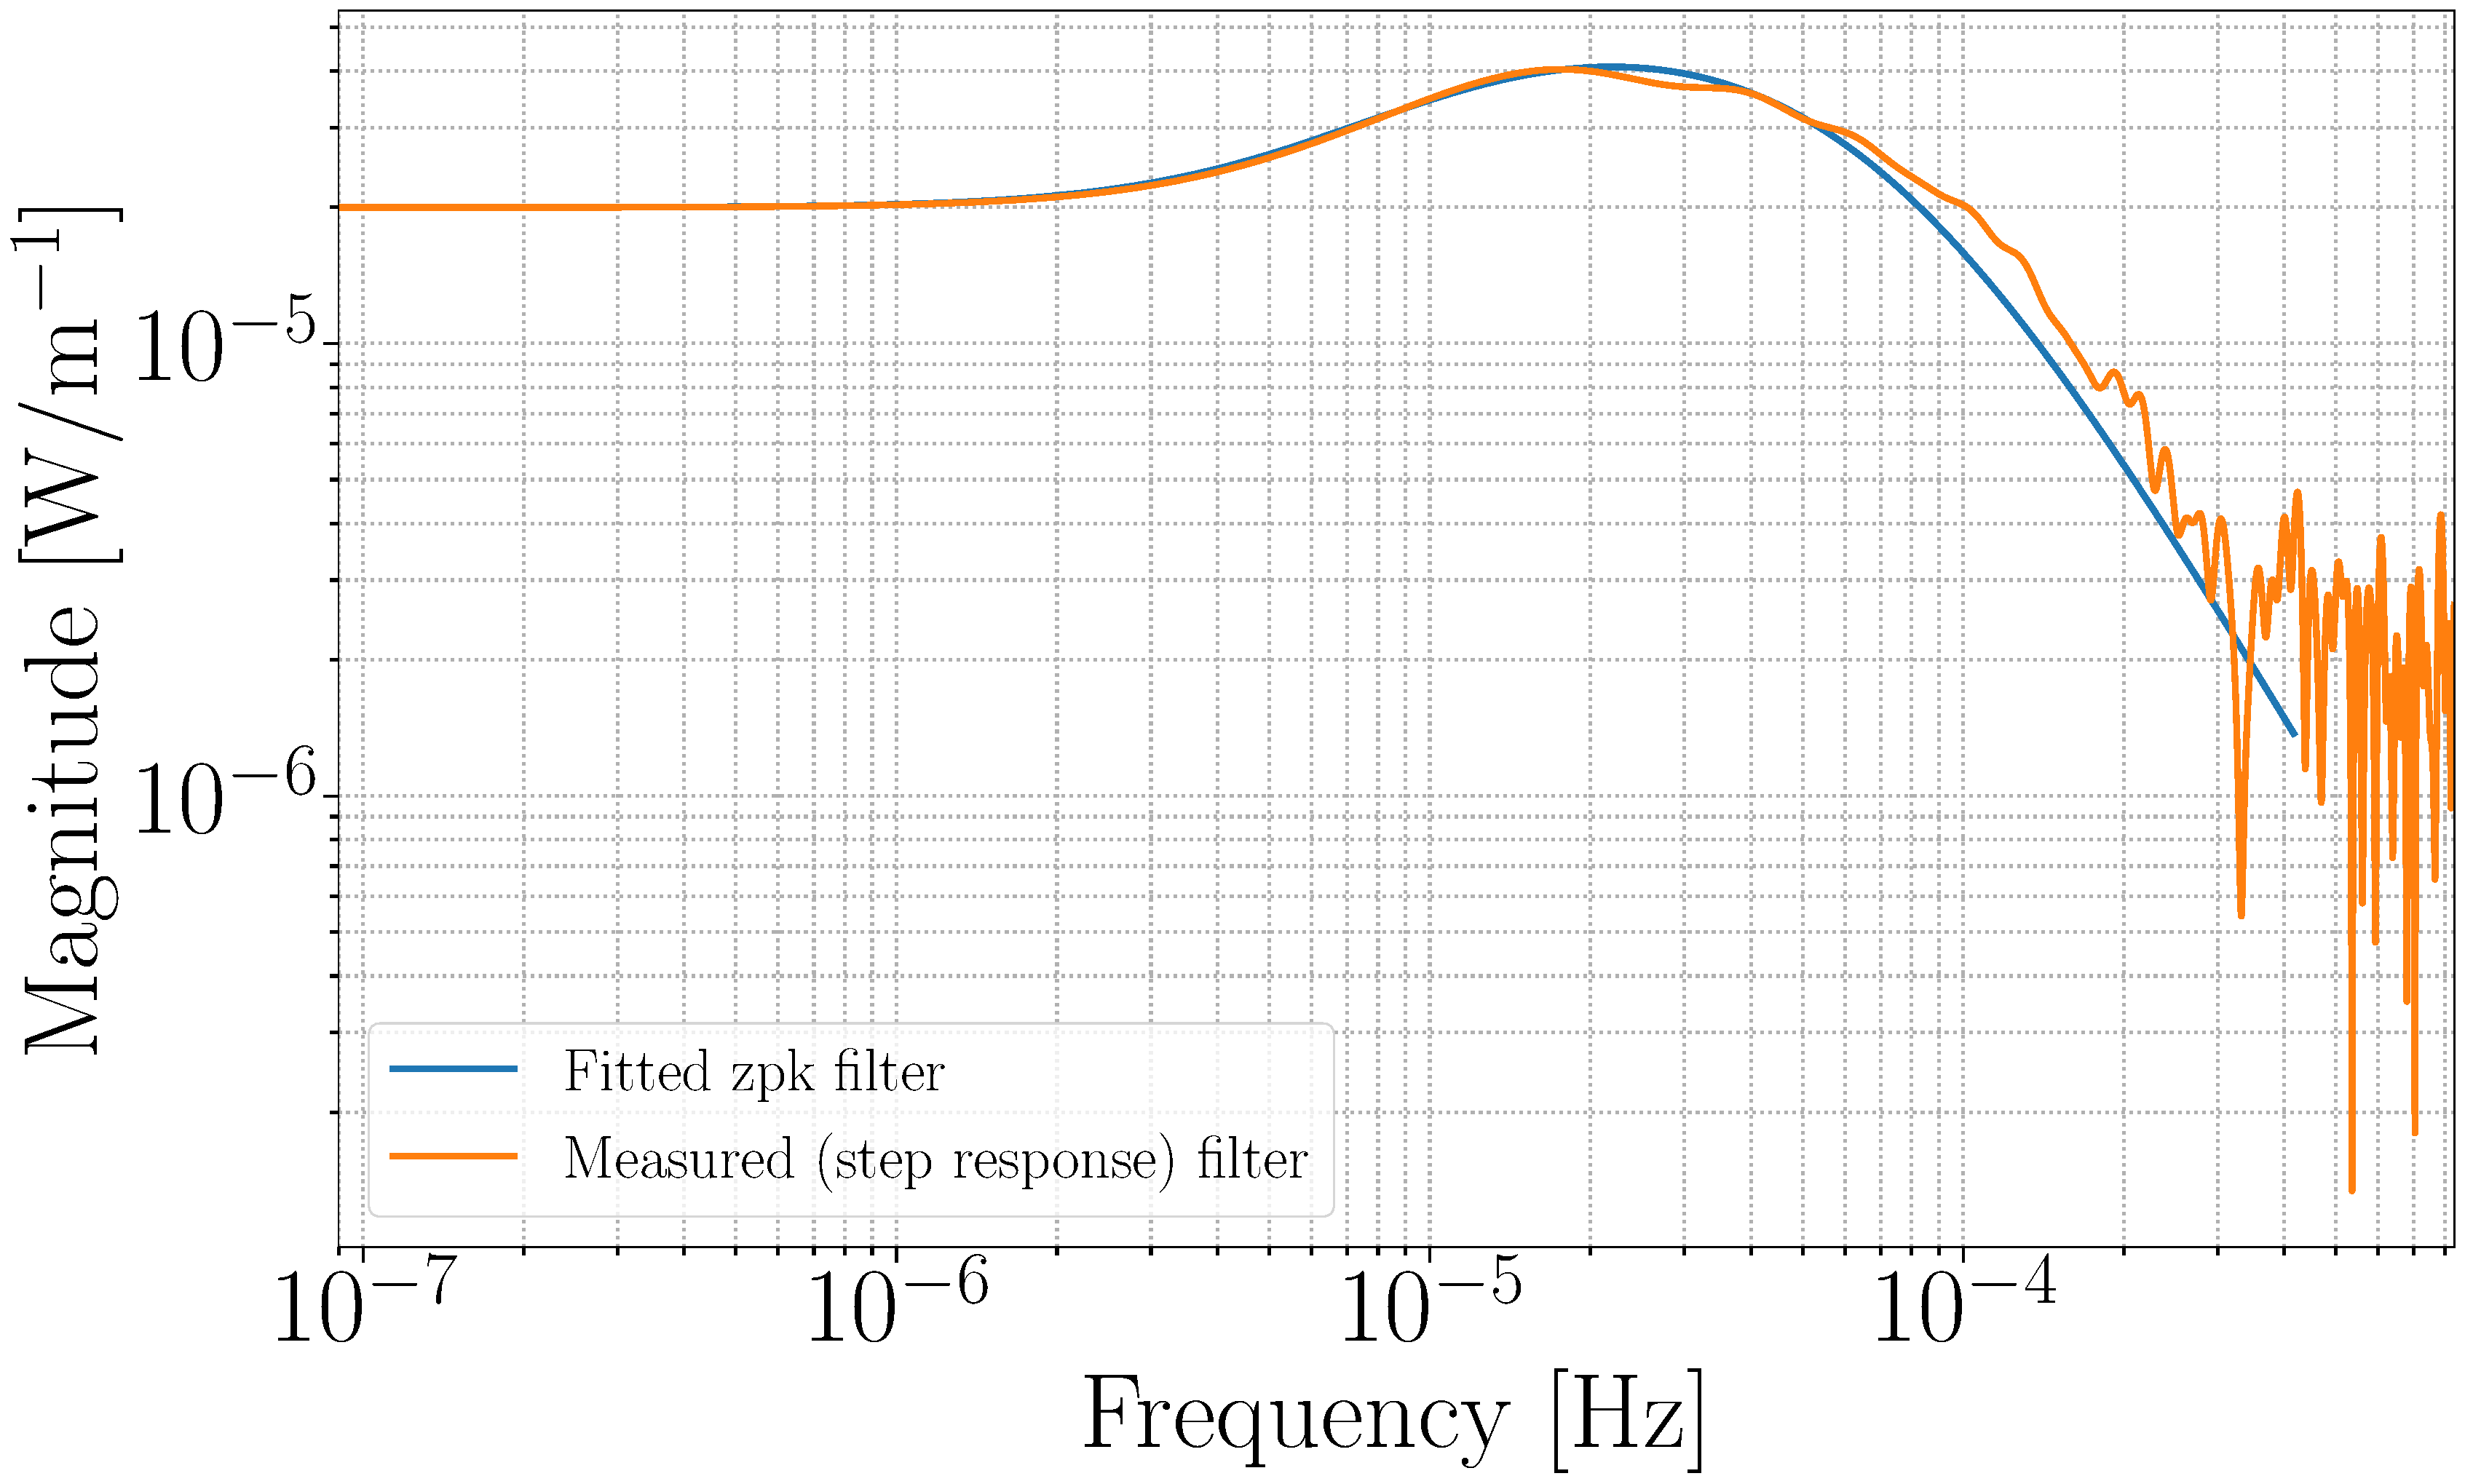
\includegraphics[width=\textwidth]{TCS/IRHF/RH_plant_filter_fit}
\caption{Showing the PSD of the RH response (normalized by the input RH power) over a an $\approx$ 12.5 hour period. The zpk model of the fitted filter (H(s)) is $9.2545e-12 \frac{(s+3.14210e-5)}{(s+8.168e-5)(s+0.0003142)(s+0.0005969)}$}
\label{fig:plant_v_fit}
\end{figure}

\begin{figure}[H]
\centering
\includegraphics[page=2,width=.9\textwidth]{TCS/IRHF/RH_input_filter_figures.pdf}
\caption{A pictograph showing the system with real time digital filtering for an improved thermo-optic response. The RH input filter is created by inverting the plant filter combine with a low pass and added poles to the zpk model to ensure stability.}
\label{fig:rtdf_pictograph}
\end{figure}

\subsection{Dynamic Thermal compensation}
\begin{figure}[H]
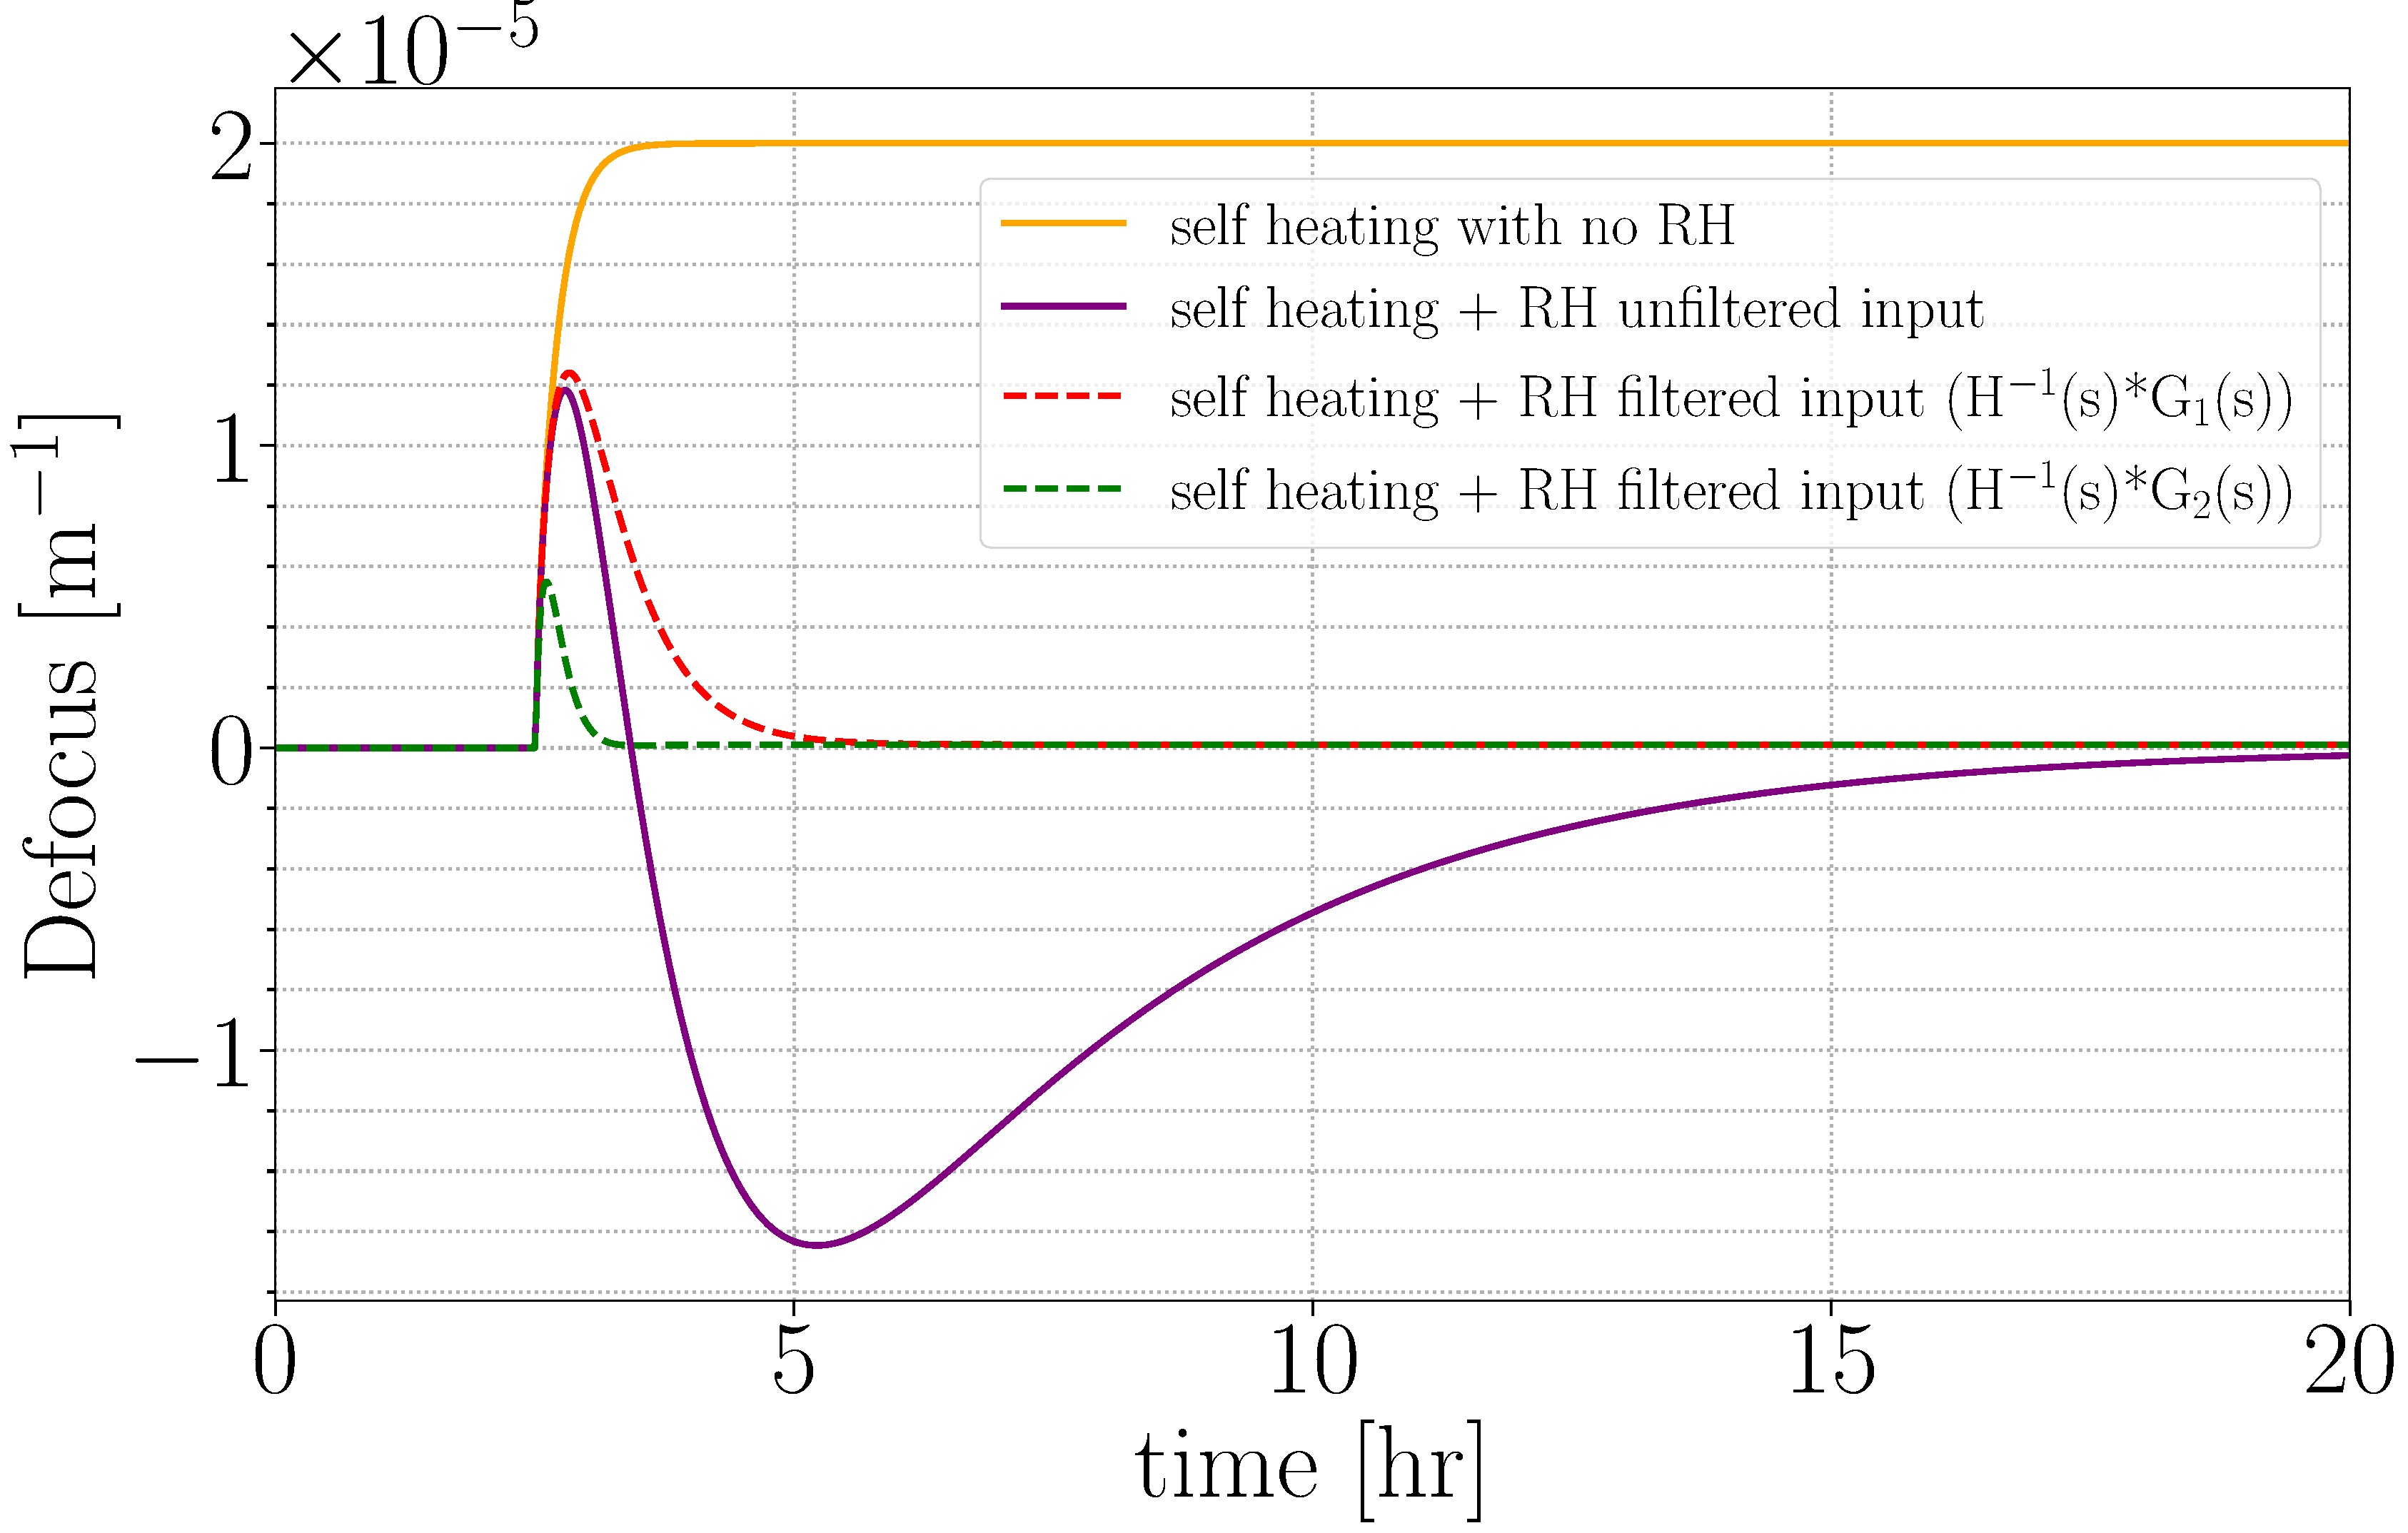
\includegraphics[width=\textwidth]{TCS/IRHF/IRHF_compare_w_self}
\caption{Comparison of the natural RH response and the response to the conditioned input. The above plot is simulated in Matlab by passing the RH input time series (top plot) through the $[H(s)]^{-1*}$ and $H(s)$ to acquire with the result lensing behavior on the bottom plot.}
\label{fig:dynam_comparison}
\end{figure}
\newpage


\subsubsection{Limitations}
\begin{figure}[H]
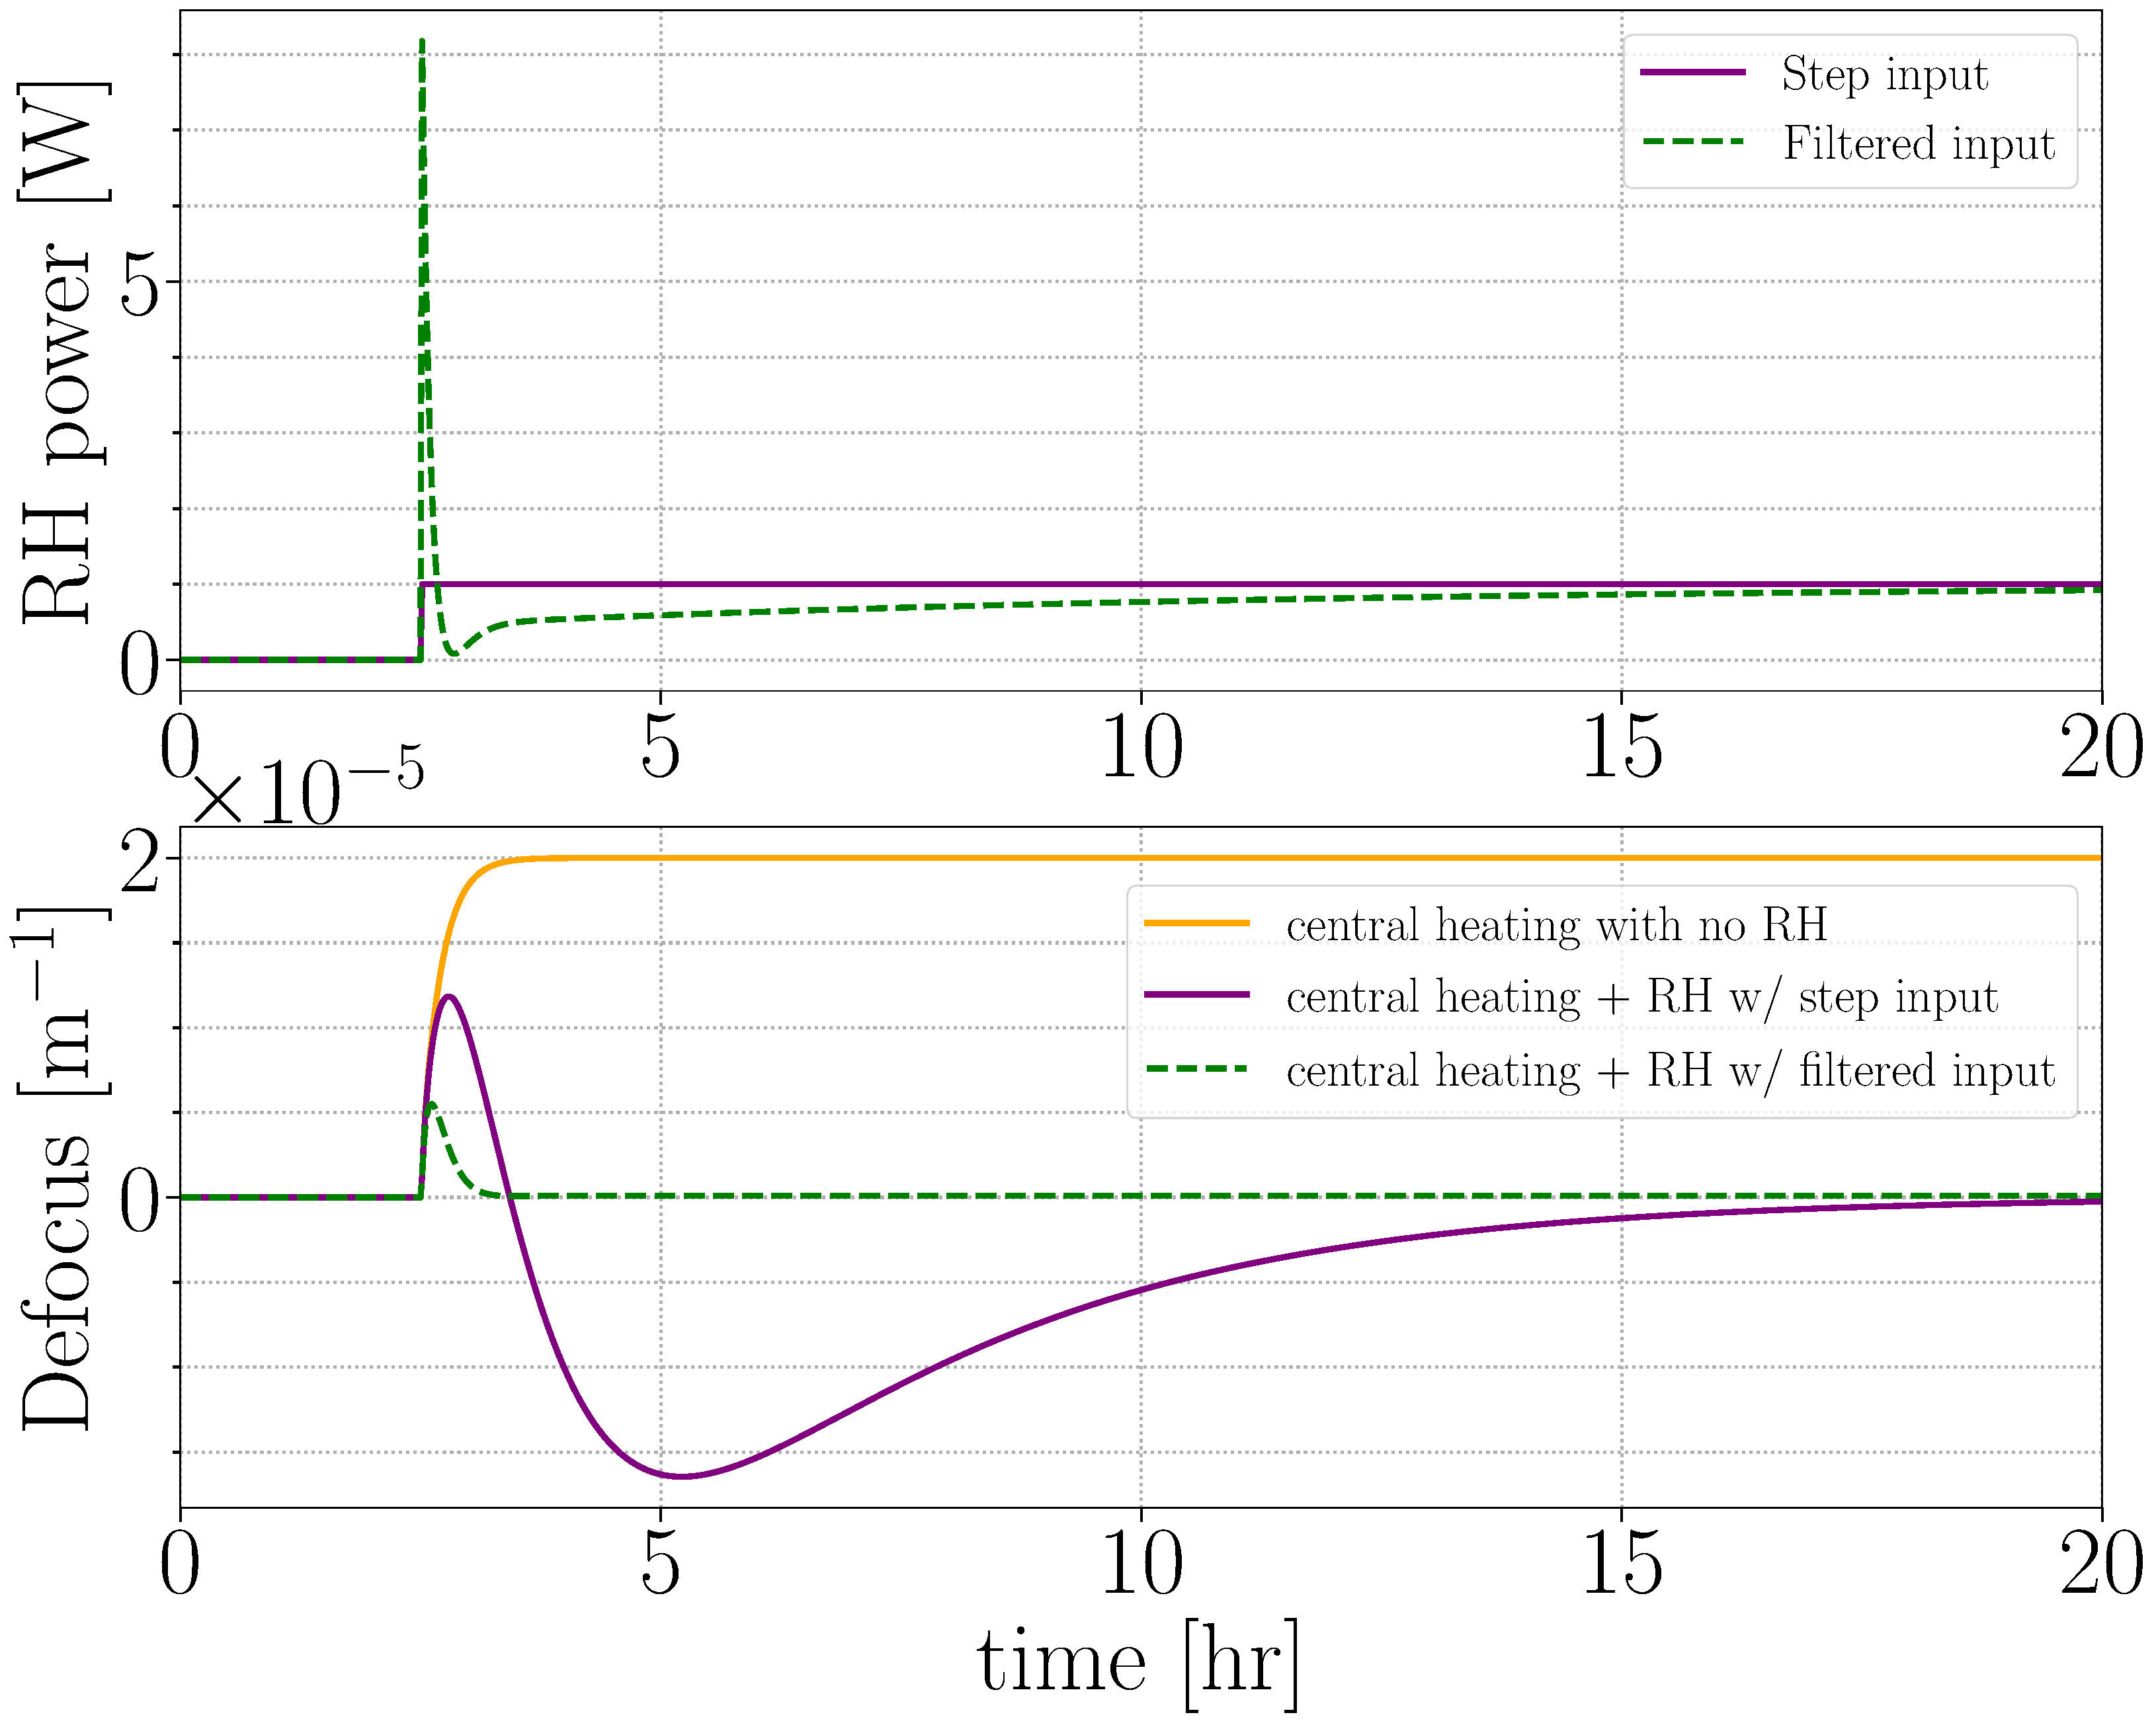
\includegraphics[width=\textwidth]{TCS/IRHF/IRHF_compare_filts_PI_paper}
\caption{Comparison of the natural RH response and the response to the filtered input with RH power}
\label{fig:RH_power}
\end{figure}
Limitation on RH power is set at 8W \textcolor{red}{Double check source?}

\textcolor{red}{Implementation into CDS at LHO (appendix?)}


\section{Point absorbers in O3a}

\begin{itemize}
\item Impact on RF sidebands with interferometer thermalization
\end{itemize}

\subsection{Studies}

\subsection{Actuation using a $\mathrm{CO_2}$ laser and mask}
\begin{itemize}
\item Aiden's design
\item Imaging
\item Installation
%\begin{figure}[H]
%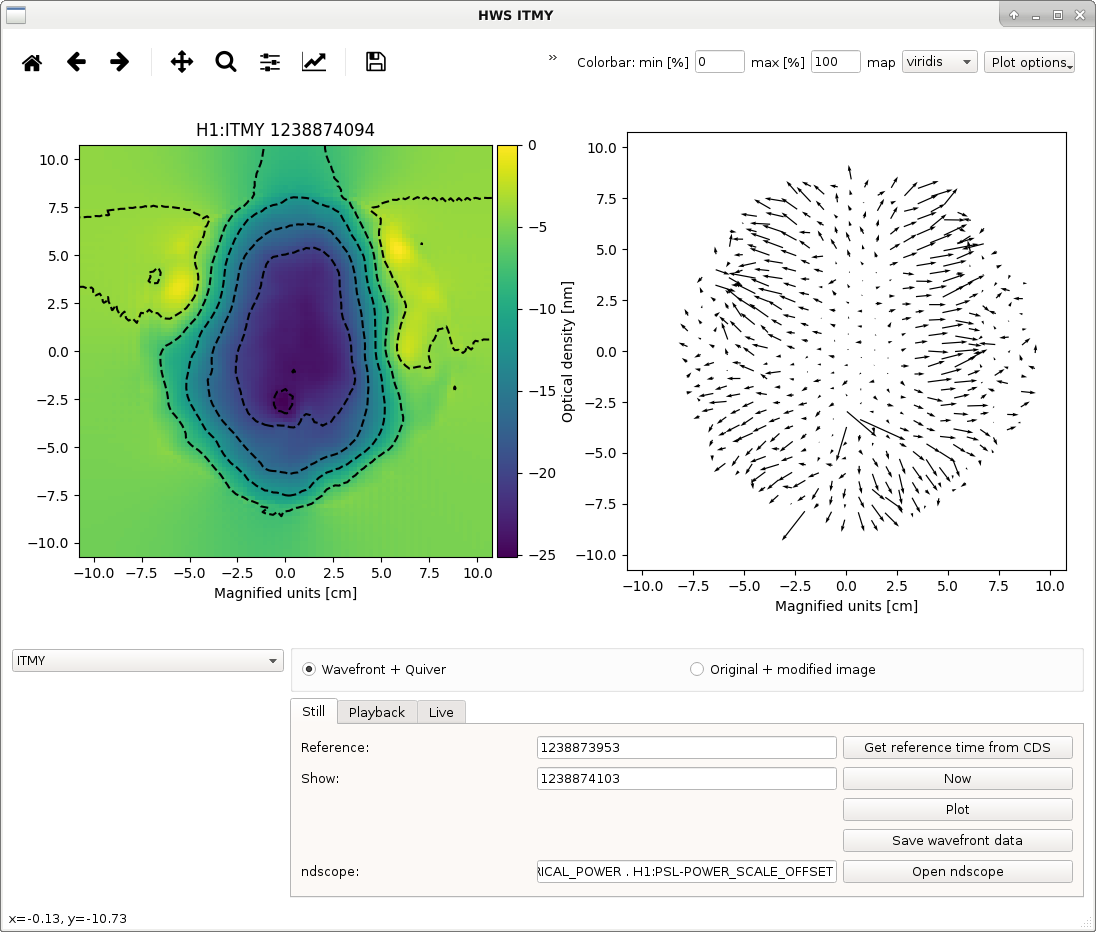
\includegraphics[width=\textwidth]{figs/TCS/PA/48349_20190409201649_inital_install_CO2Ymask2_150seconds_900mW.png}
%\caption{Point absorber figure with second $\mathrm{CO_2}$ mask}
%\label{fig:RH_power}
%\end{figure}

\item Metric of improvement? (Impact on sidebands after thermalization) (Tracking dither line amplitudes)
\end{itemize}
